\section{Metode Penelitian} % Dapat diganti menjadi "Kerangka Pikir" jika perlu

%=========================================================%
%           TULIS METODE/KERANGKA PIKIR DI SINI           %
% Jangan Lupa untuk Menghapus Contoh Tulisan di Bawah Ini %
%=========================================================%

Data yang digunakan dalam penelitian ini adalah data sekunder, berupa data Karakteristik Mahasiswa Universitas Terbuka Program Studi Statistika Tahun 1009.1 s/d 2019.2. Data terbagi menjadi dua, yaitu data \textit{training} 1046 mahasiswa dan data \textit{testing} 447 mahasiswa yang diambil untuk penerapan metode JST \textit{Backpropagation}, seperti yang dapat dilihat pada \autoref{table:karakteristik-mahasiswa-stat-ut} sebagai berikut:

\begin{table}[H]
    \centering
    \caption{Karakteristik Mahasiswa Universitas Terbuka Program Studi Statistika}
    \label{table:karakteristik-mahasiswa-stat-ut}
    \begin{tblr}{colspec={c l c l}, hline{1,2,Z}={1-Z}{solid}, row{1}={font=\bfseries}}
        Variabel & Keterangan & Skala Pengukuran & Kategori \\
        \SetCell[r=2]{} $X1$ & \SetCell[r=2]{} Jenis Kelamin & \SetCell[r=2]{} Nominal & 1 = Pria \\
             &               &         & 2 = Wanita \\
        $X2$ & Usia & Interval & \\
        \SetCell[r=5]{} $X3$ & \SetCell[r=5]{} Pendidikan & \SetCell[r=5]{} Ordinal & 1 = SLTA/SMK \\
             &            &         & 2 = Diploma \\
             &            &         & 3 = S1 \\
             &            &         & 4 = S2 \\
             &            &         & 5 = S3 \\
        \SetCell[r=2]{} $X4$ & \SetCell[r=2]{} Status Pernikahan & \SetCell[r=2]{} Nominal & 1 = Belum Menikah \\
             &                   &         & 2 = Menikah \\
        \SetCell[r=5]{} $X5$ & \SetCell[r=5]{} Status Pekerjaan & \SetCell[r=5]{} Nominal & 1 = Tidak Bekerja \\
             &                  &         & 2 = Karyawan Swasta \\
             &                  &         & 3 = Wiraswasta \\
             &                  &         & 4 = PNS \\
             &                  &         & 5 = TNI/Polri \\
        $X6$ & Tahun Registrasi Awal & Interval & \\
        $X7$ & Jumlah Registrasi & Internal & \\
        $X8$ & SKS Tempuh & Interval & \\
        $X9$ & IPK & Interval & \\
        \SetCell[r=2]{} $Y$ & \SetCell[r=2]{} Status Mahasiswa & \SetCell[r=2]{} Nominal & 0 = Tidak Aktif \\
             &                  &         & 1 = Aktif
    \end{tblr}
\end{table}

\autoref{fig:flowchart-jstb} di bawah ini merupakan gambar \textit{flowchart} metode JST \textit{Backpropagation}:

\begin{figure}[H]
    \centering
    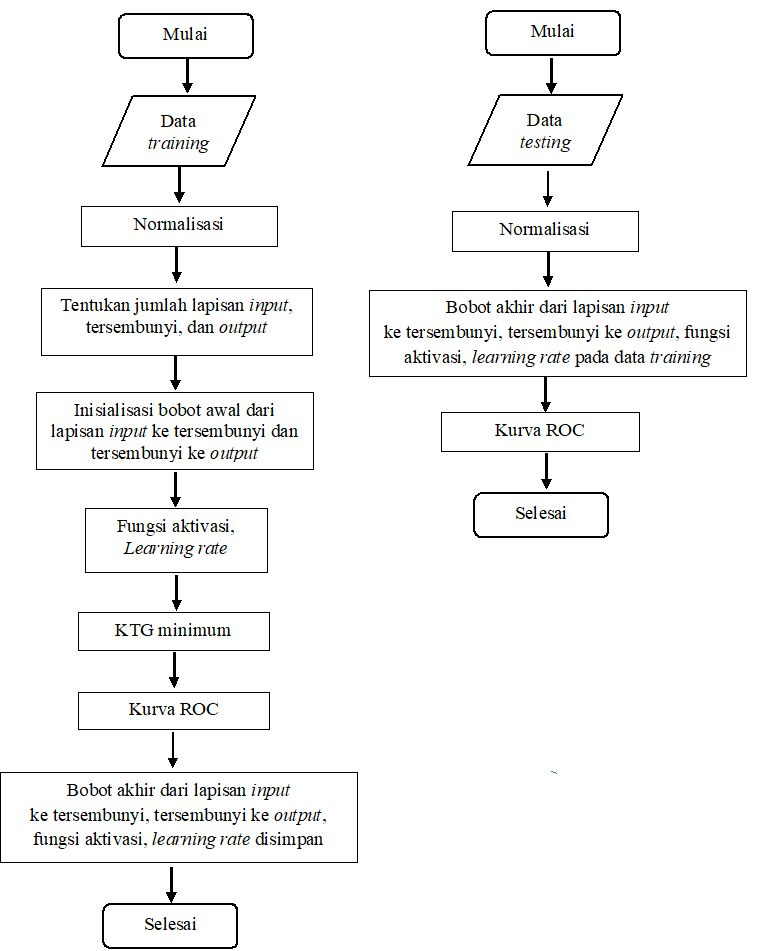
\includegraphics[width=.6\linewidth]{image/Flowchart JST Backpropagation.jpg}
    \caption{\textit{Flowchart} JST \textit{Backpropagation}}
    \label{fig:flowchart-jstb}
\end{figure}